\section{Floating Platform}
The floating platform, depicted in
\cref{fig:floatingPlatform}, is the main structure of the built vehicle.
It is a baffle of glulam, with two pieces of XPS cell foam as
pontoons, which all components are attached to. It can keep a mass of
around 20~kg above the water surface.% with margins.

In the middle of the platform two symmetrical holes with fittings has
been made, in which the RBR modules can be attached or detached. In the front of the platform, a large rounded bumper helps deflecting head on collisions. It also creates a distance between the platform and
any side obstacles, which facilitate manoeuvring in tight spots and corners. The majority of the electronics were placed in the middle of the platform. The electronics and the RBR modules have acrylic
covers, protecting the equipment from rain and small splashes of water.

\begin{figure}[h]
   \centering
   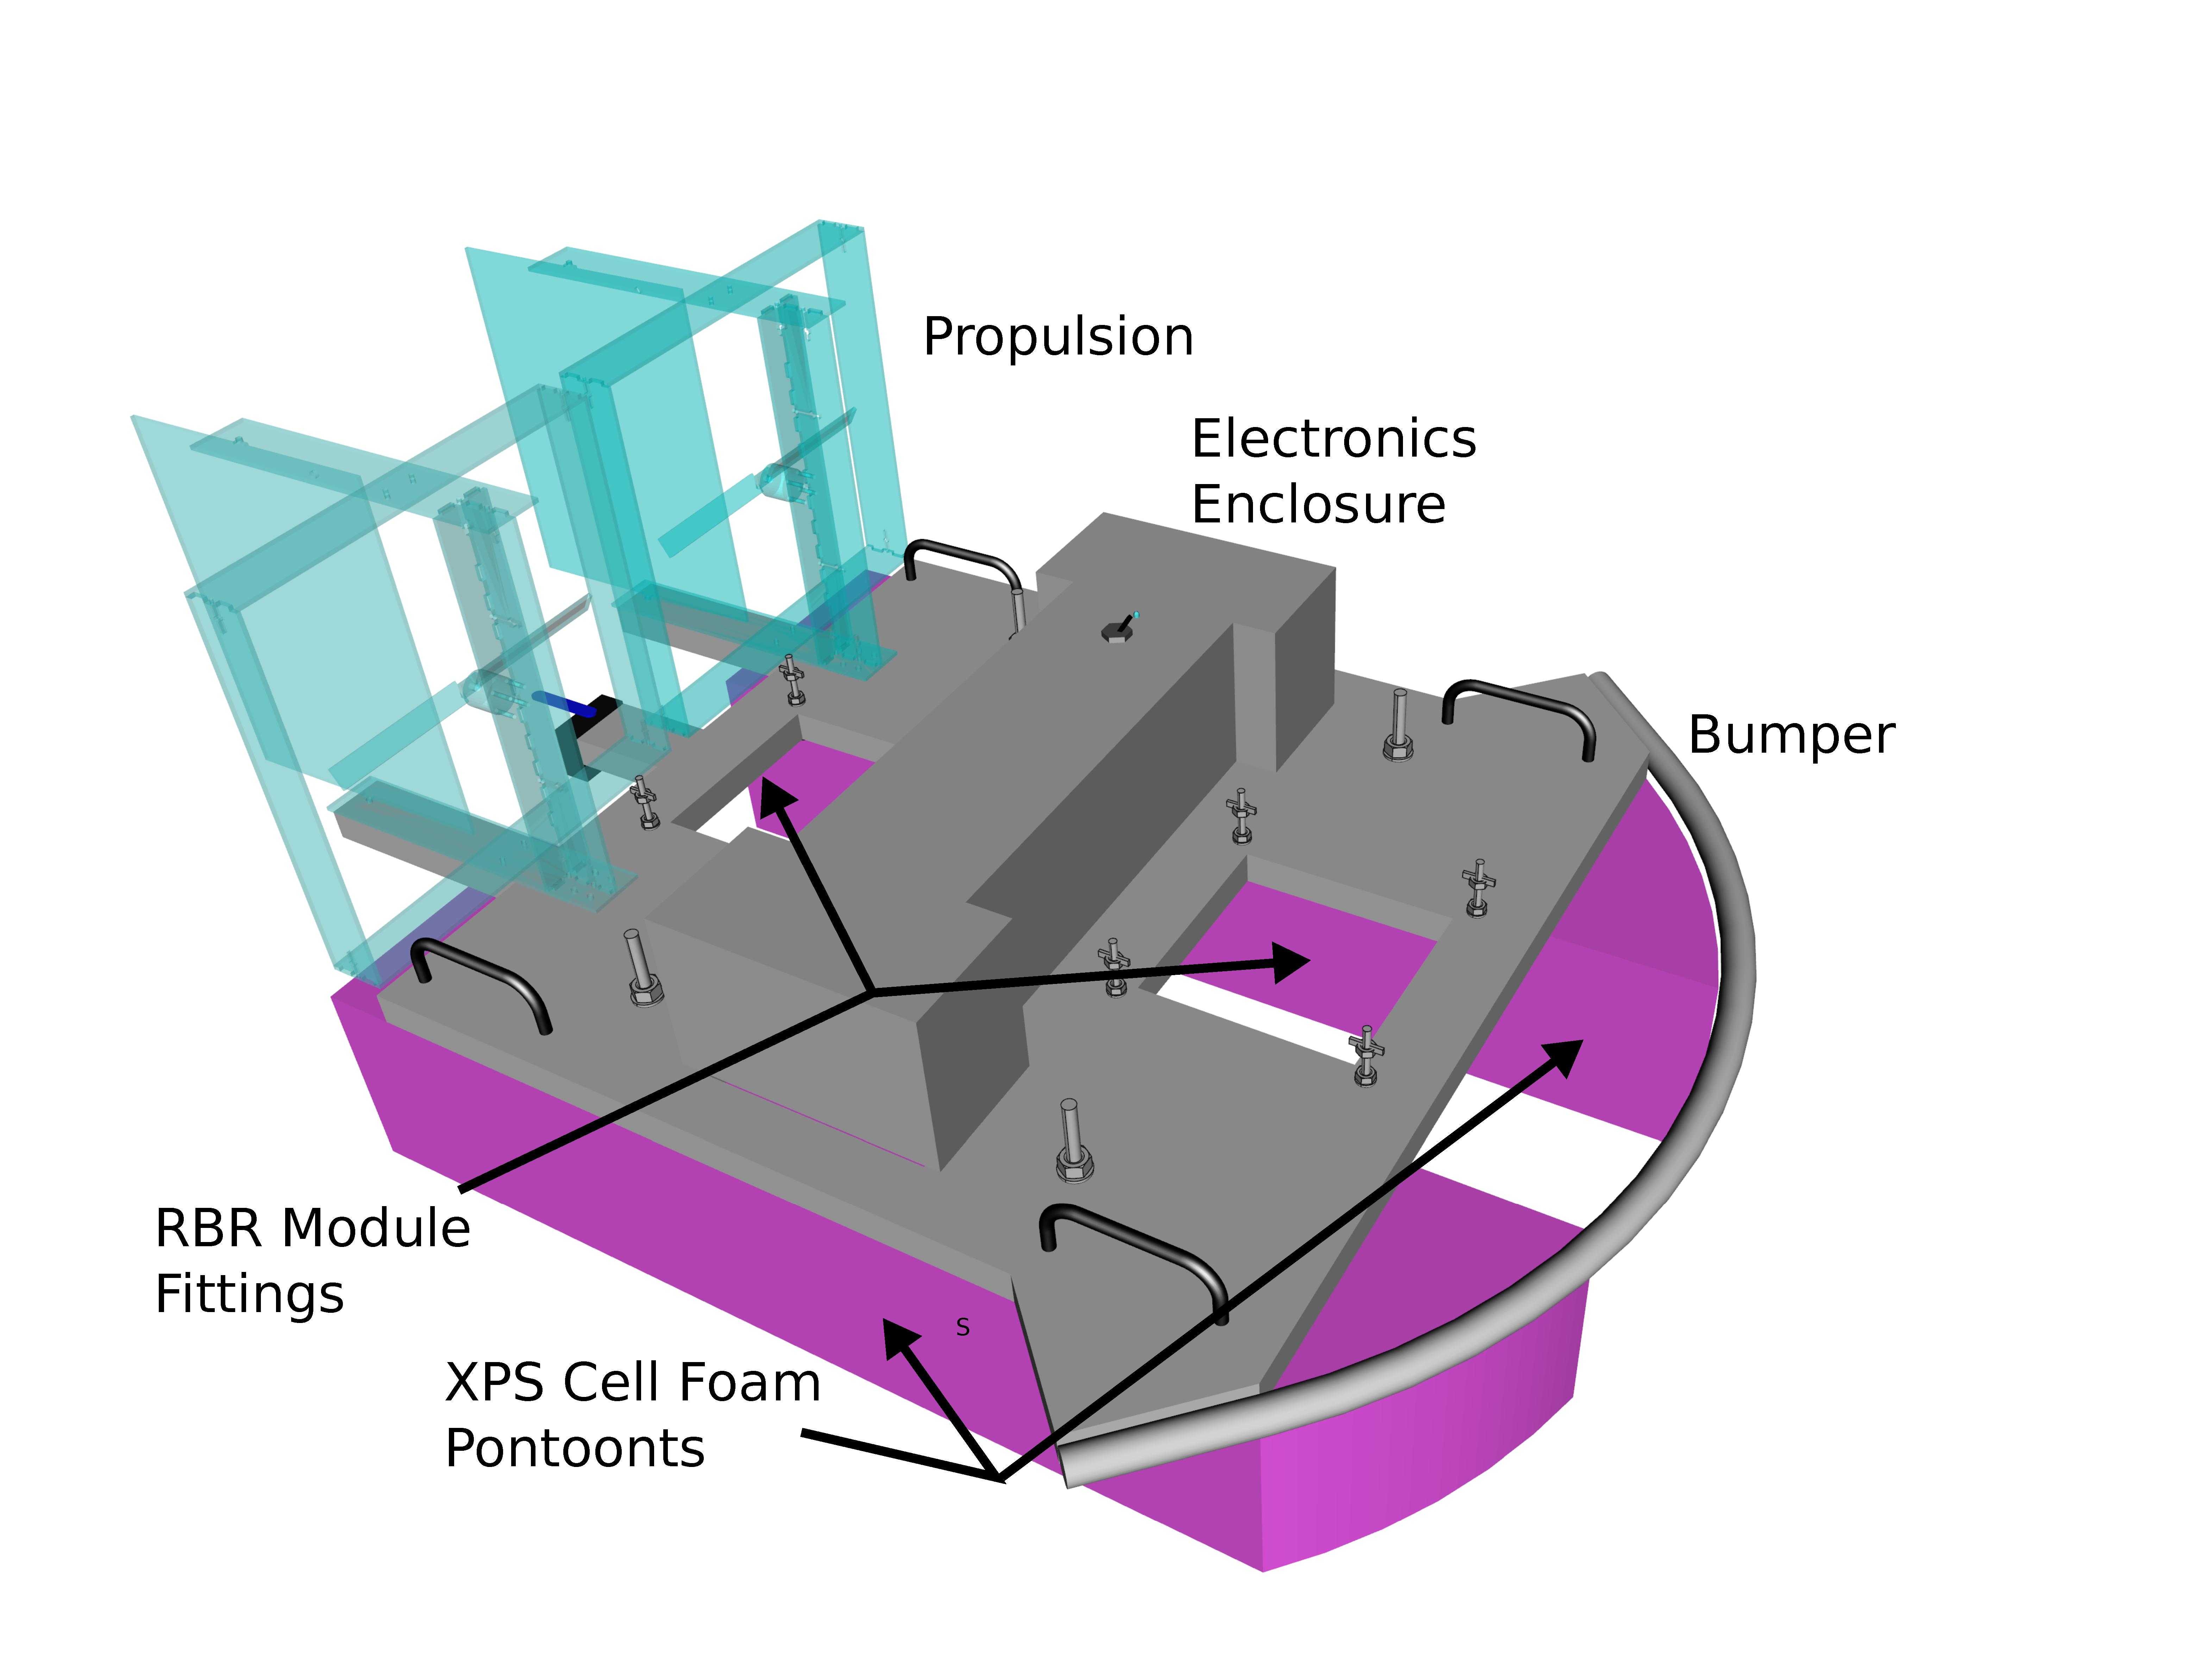
\includegraphics[width=.75\textwidth]{platformWithNotes.eps}
   \caption{The floating platform without the RBR modules installed.}
   \label{fig:floatingPlatform}
\end{figure}

\subsection{RBR module}
The RBR module, seen in fig. \ref{fig:rbr-module}, consist of two plates, separated by three adjustable threaded
rods. The upper mounted plate is constructed with a modified hand-held screwdriver. The lower mounted
plate has a PTFE shaft guide mounted to hold the RBR axle in place. The axle can be driven through the shaft guide and be attached to the screwdriver, in order to rotate the RBRs. The lower mounted baffle has an
additional wave baffle which goes down into the water just above where a mounted RBR
will be situated. This wave baffle prevents the formation of large vortices above the RBR. 

\begin{figure}[H]
  \centering
  \textbf{RBR module}
  \par\medskip
  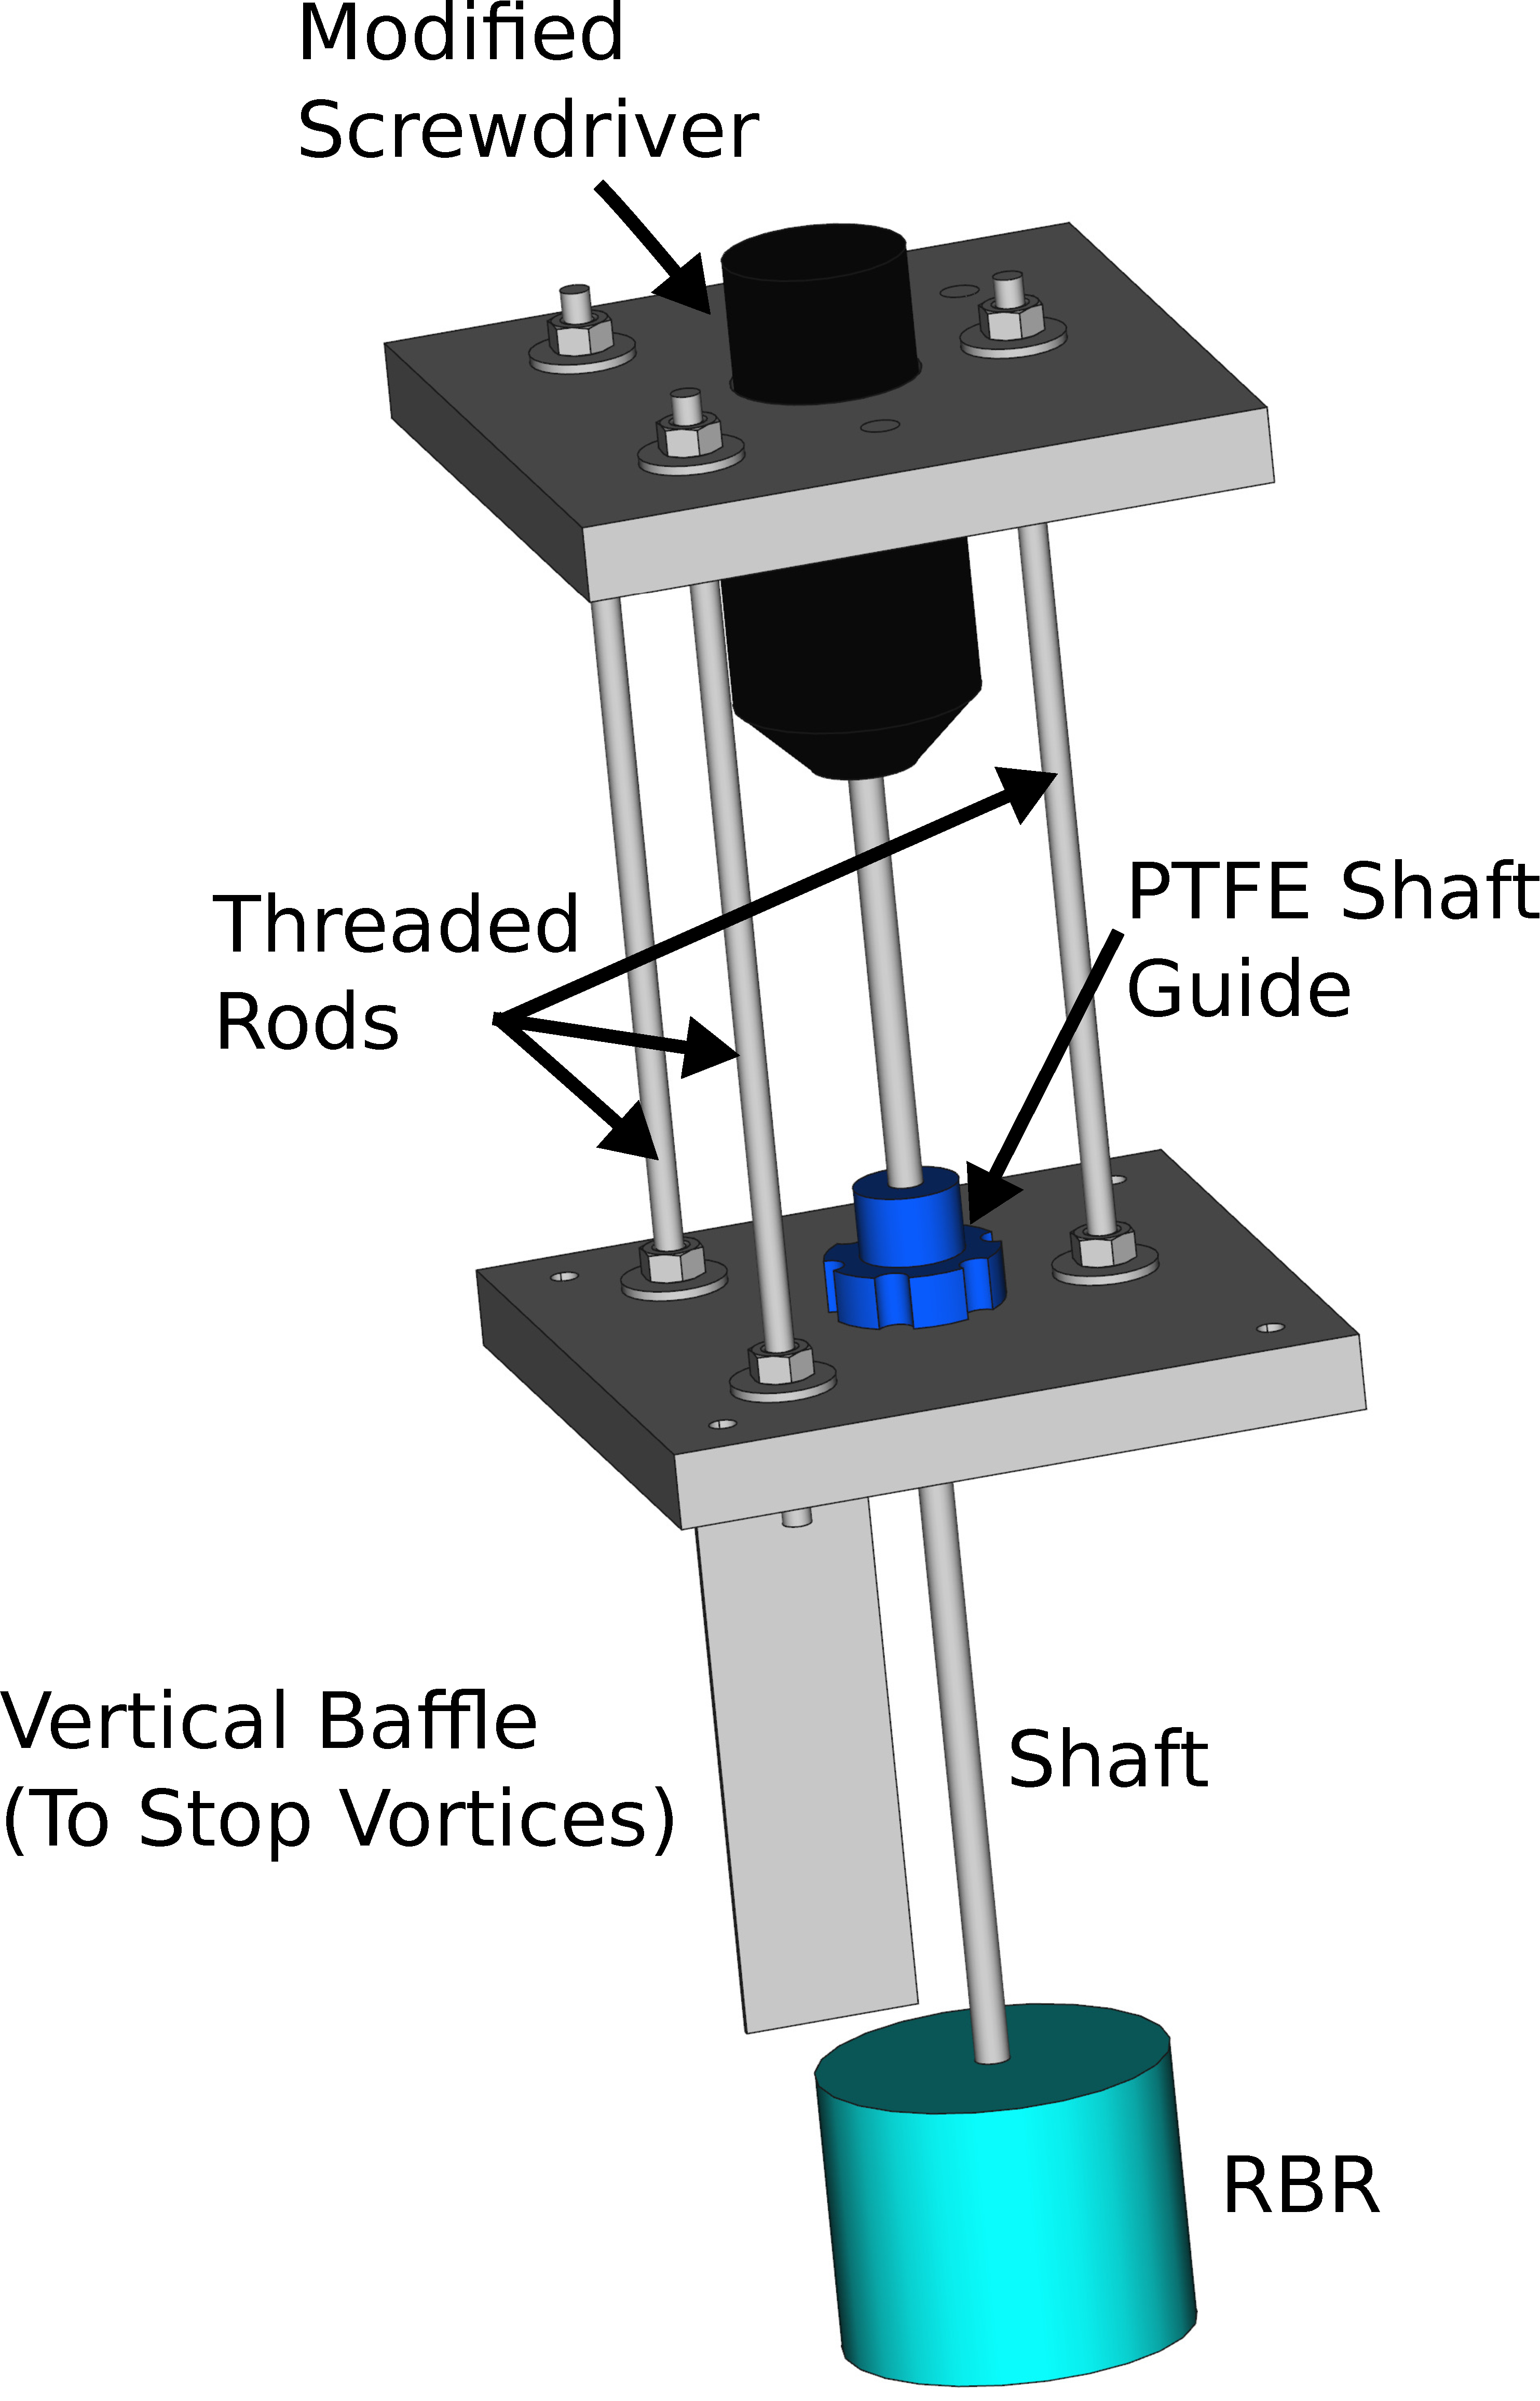
\includegraphics[width=0.5\textwidth]{RBR-moduleWithNotes}
  \caption{A RBR module with a drive assembly mounted at the top plate,
    which in turn is mounted with adjustable threaded rods to the lower plate. This houses the shaft guide for the RBR axle. The lower plate mounts to the
    top of the platform, and on the RBR modules underside sits a wave baffle.}\label{fig:rbr-module}
\end{figure}

The upper baffle can be height adjusted, in order to easily calibrate the desired depth of the RBR. To prevent air from reaching the RBRs, it is preffered to have them at a lower level than the bottom of the pontoons.
%It is ideal to have the RBR distanced from the water surface. It is preferred to have it at a lower level than the bottom of the pontoons to prevent air reaching the RBR. 


The speed of the RBRs can be controlled remotely, with a rotational speed interval ranging from 0 to 600 rotations per minute (rpm) , where 500~rpm is ideal.
%The speed of the RBRs can be controlled remotely. The rotational speed interval of the RBR ranges from 0 to 600 rpm, where 500~rpm is ideal.


The RBR modules can be attached to the intended slots on the platform, and the modules should be oriented such that the wave baffle is parallel to the travel direction, minimizing the vehicles water friction. Fly nuts are used to hold the modules in the slots. 

\subsection{Propulsion}
The propulsion made from air-propellers, was installed in an acrylic plastic protection housing. Acrylic plastic rudders were installed in front of the propellers, these are controlled through a single servo located at the back of the platform. The layout of the propulsion mechanism is shown in \cref{fig:propellerWithNotes}.

\begin{figure}[h]
   \centering
   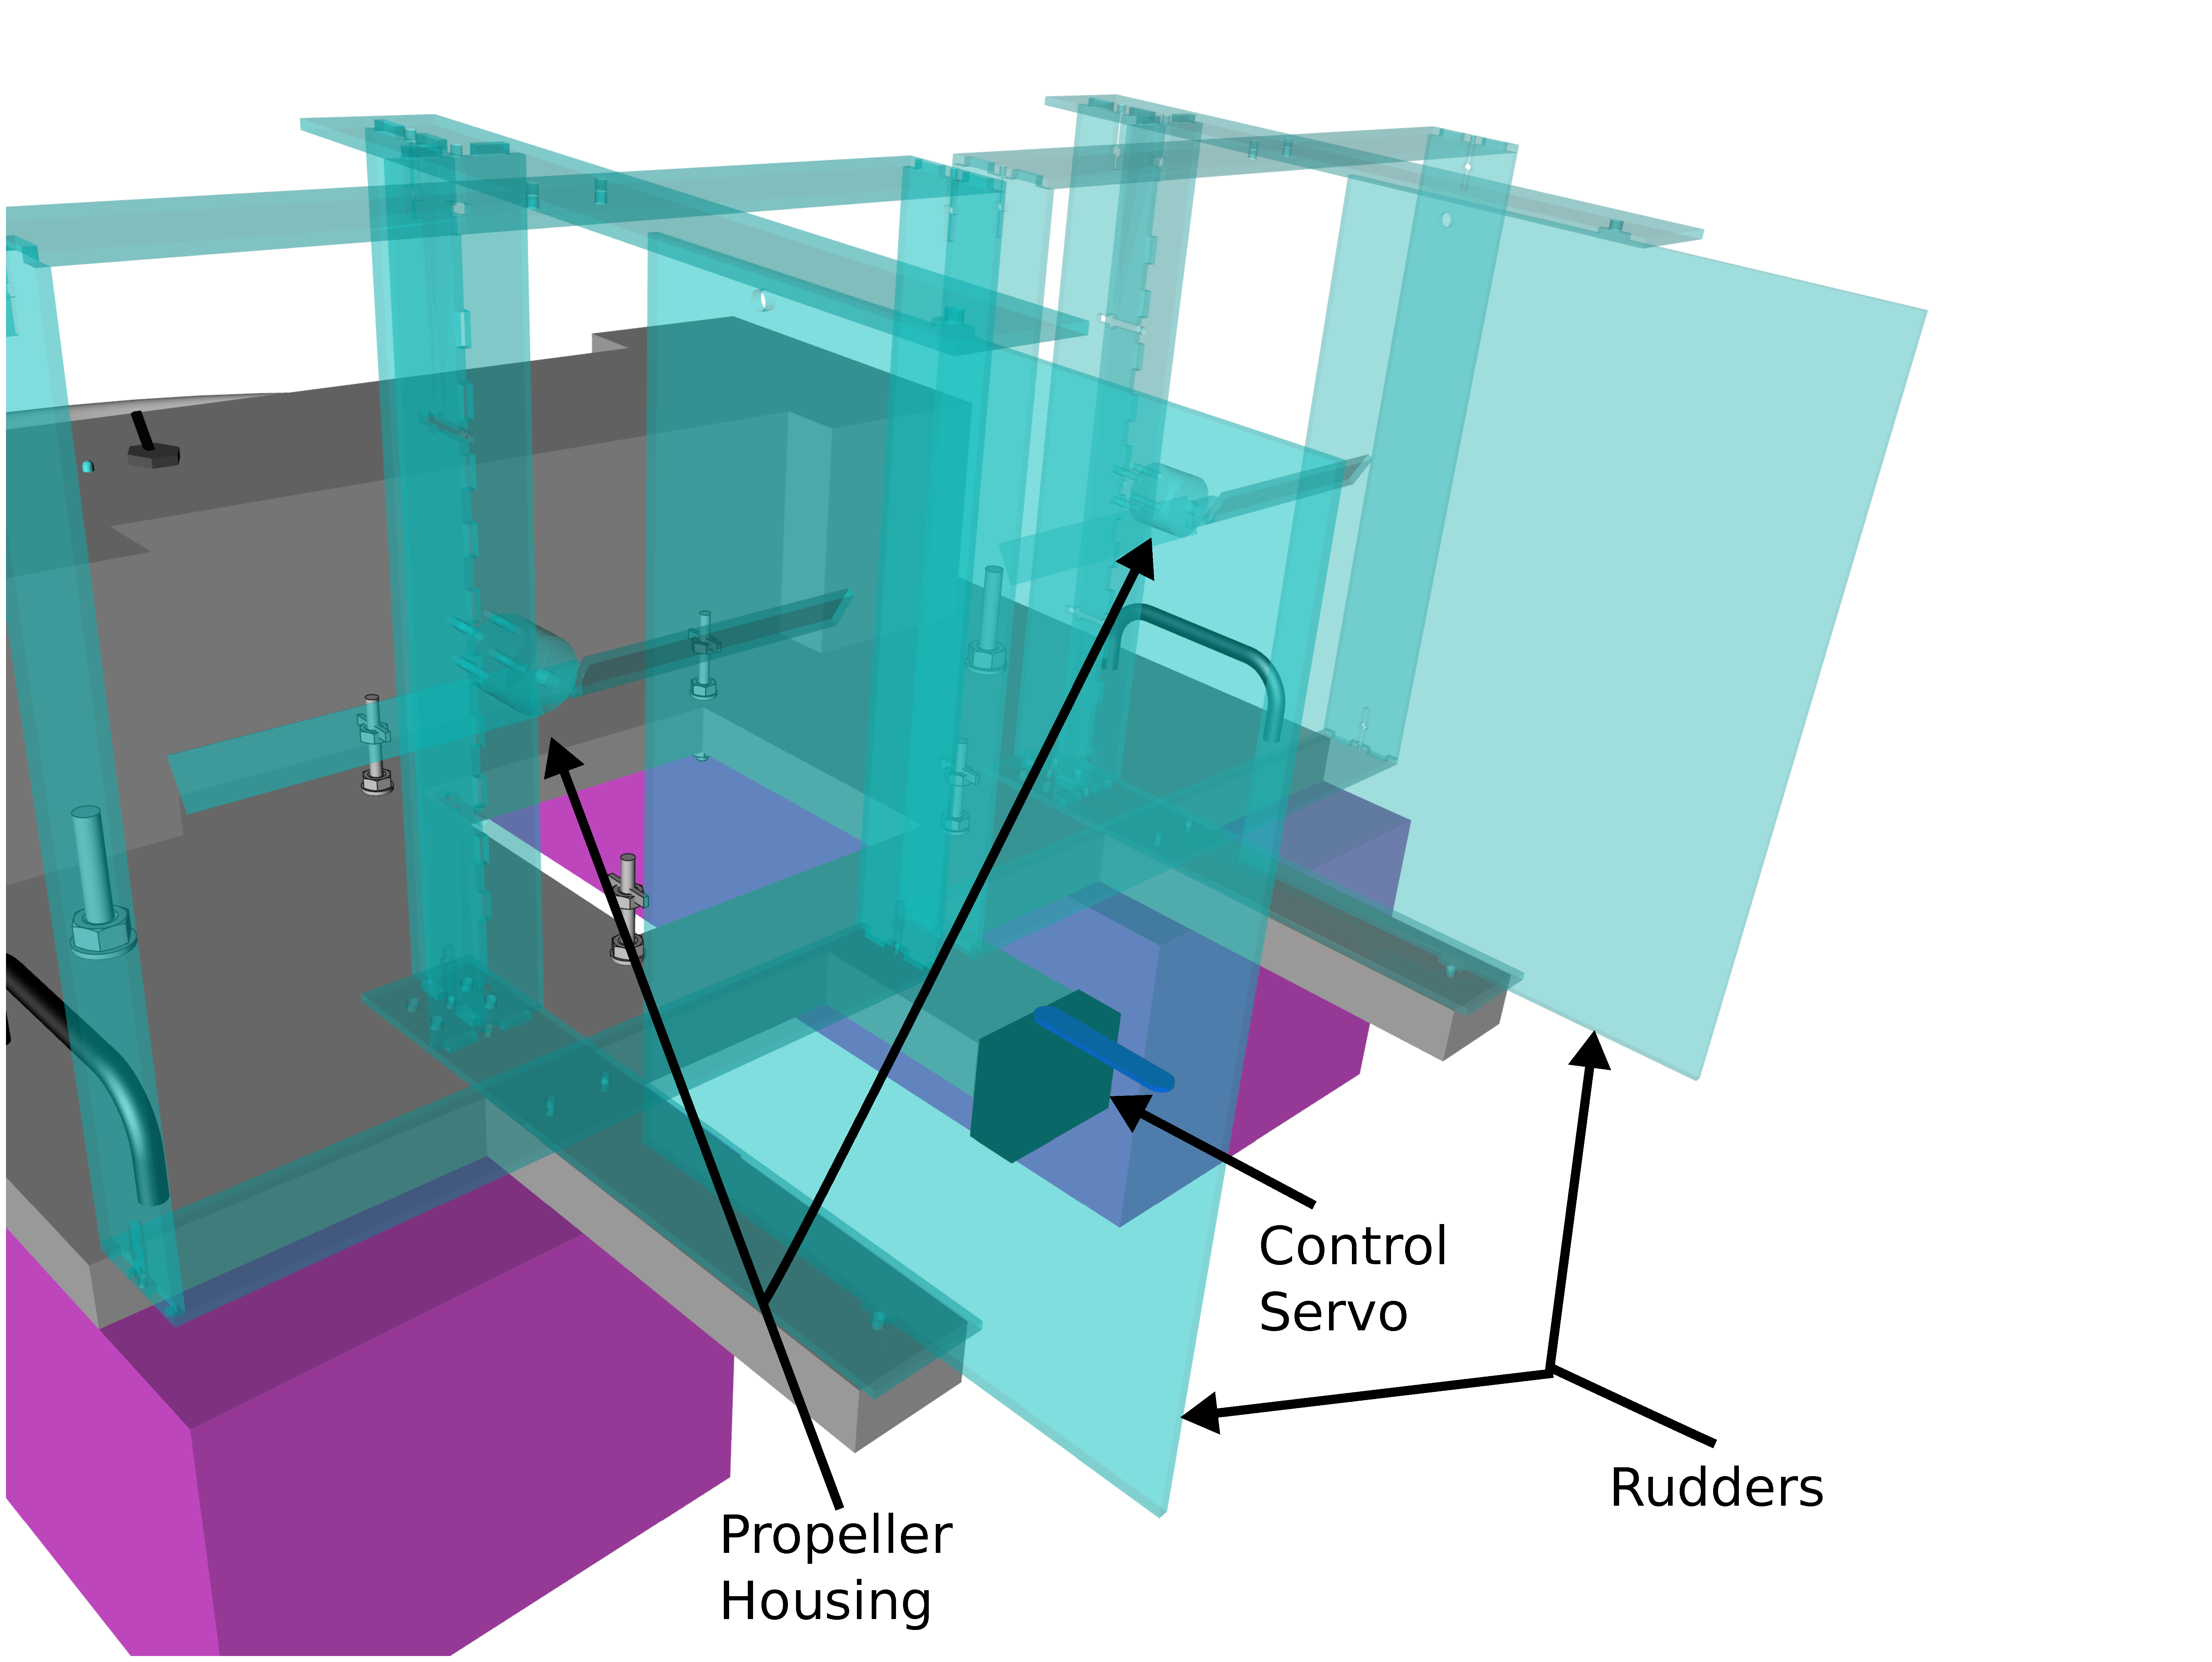
\includegraphics[width=.75\textwidth]{propellerWithNotes}
   \caption{The propulsion construction.}
   \label{fig:propellerWithNotes}
\end{figure}

\subsection{Water protection}

An acrylic protection cover was manufactured in order to protect the batteries, the engine control units, and other electronic equipment. Two separate acrylic covers were also constructed to protect the drive assemblies of the RBR modules. These covers do not protect the equipment from submersion, only from rain and small splashes of water. %To install the covers, just place them over the RBR modules. 
The cover for the electronics is held in place with one screw on either side of the electronic enclosure.

\subsection{Transportation}

To ease transportation, the weight of the platform can easily be reduced. This can be done by first removing the protective covers, followed by disconnecting the power cables connected to the batteries and RBR drive assemblies. It is then possible to remove the batteries and RBR modules from the platform. Since the propulsion mounts are made of semi-thin acrylic pieces, care needs to be taken during transports. %During transport care needs to be taken such that the propulsion mounts are not damaged, as these parts are fragile.
%%% Local Variables: 
%%% mode: latex
%%% TeX-master: "document"
%%% End: 
